\section*{Exercice 189 -- Schéma-Blocs et FT}
\setcounter{exo}{0}
%CCS PSI 2025

On considère l'asservissement angulaire d'un axe numérique. On note $\Delta \theta_1$ la grandeur asservie.
%On appelle «~axe $i$~» l’axe associé à la grandeur asservie $\Delta \theta_i$. La structure retenue pour l’asservissement est
%identique pour les deux axes. L’étude est restreinte à la conception du correcteur de l’axe 1.

\textbf{Hypothèses, notations et paramétrage}

\begin{itemize}
\item Les conditions initiales sont nulles.
\item L'équation du mouvement de l’axe est donnée par : $\Delta C_1(t) = J \dfrac{\dd^2 \Delta \theta_1(t)}{\dd t^2}-k_1 \dfrac{r_9'}{r_0}h_2 \Delta F_x(t)$ avec $J=\SI{1,98e-5}{kg.m^2}$, $k_1 \dfrac{r_9'}{r_0} = 0,00717$, $h_2=\SI{0,2}{m}$. 
\item Le couple moteur $\Delta C_1(t)$ est fourni par une machine à courant continu modélisée par les équations suivantes : $u_1(t)=L\dfrac{\dd i_1(t)}{\dd t}+Ri_1(t) + e_1(t)$, $e_1(t)=k_e \dfrac{\dd \Delta \theta_1(t)}{\dd t}$, $\Delta C_1(t)=k_t i_1(t)$ avec $u_1(t)$ la tension aux bornes du moteur, $i_1(t)$ l’intensité traversant le moteur et $e_1(t)$ la force contre
électromotrice, avec $R=\SI{2,07}{\Omega}$,
$k_t=\SI{0,0525}{N.m.A^{-1}}$, $k_e=\SI{0,0525}{V.s.rad^{-1}}$.
\item On fait l’hypothèse que l’influence de l’inductance $L$ est négligeable sur les performances attendues, soit $L=\SI{0}{H}$.
\item La consigne est notée $\Delta \theta_{c1}(t)$.
\end{itemize}

Le cahier des charges sélectif conduit à choisir un correcteur associant une anticipation (via la présence de $\sigma_4$ dans la relation suivante) et une correction PID. La tension de commande du moteur est donnée par : 
$U_1(p)=\left( \Delta \theta_{c 1}(p)  - \Delta \theta_{1}(p)  \right) \left( \sigma_1 +\dfrac{\sigma_2}{p}\right) - \sigma_3 p \Delta \theta_1(p) + \sigma_4 \Delta \theta_{c1}(p)
 $

avec $\Delta \theta_{c1}(p)$ la consigne de position angulaire exprimée dans le domaine symbolique.



\subparagraph{}
\textit{Compléter le schéma bloc du document réponse (forme littérale des fonctions de transfert).}
\ifprof
\begin{corrige}
\end{corrige}
\else
\fi


Pour la suite, on considère la perturbation nulle $\left(\Delta F_x(p)=0\right)$.

\subparagraph{}
\textit{À partir de ce schéma-blocs, en notant $H_{\text{processus}}(p)=\dfrac{\Delta \theta_1(p)}{U_1(p)}=\dfrac{K}{p\left(1+\tau p \right)}$, exprimer $K$ et $\tau$ en fonction des données de l'énoncé, puis les calculer numériquement.}
\ifprof
\begin{corrige}
\end{corrige}
\else
\fi


\subparagraph{}
\textit{Exprimer la fonction de transfert en boucle fermée, sous forme canonique, notée $B_F(p)=\dfrac{\Delta \theta_1(p)}{\Delta \theta_{c1}(p)}$ en fonction de $K$, $\tau$, $\sigma_1$, $\sigma_2$, $\sigma_3$ et  $\sigma_4$.}
\ifprof
\begin{corrige}
\end{corrige}
\else
\fi

On pose $B_F'(p)=\dfrac{p-z_0}{\left(p-p_2 \right)\left( p-p_1\right)^2}$.



\subparagraph{}
\textit{Déterminer $K'$ tel que $B_F(p)=K'B_F'(p)$, $K'$ étant un gain constant.}
\ifprof
\begin{corrige}
\end{corrige}
\else
\fi


\subparagraph{}
\textit{Exprimer les paramètres $\sigma_1$, $\sigma_2$ et $\sigma_3$ de la relation du PID en fonction de $p_1$, $p_2$, $K$ et $\tau$.}
\ifprof
\begin{corrige}
\end{corrige}
\else
\fi


Pour information, en poursuivant le calcul, on trouve $\sigma_4 = \dfrac{\tau }{K}\left( \dfrac{p_1^2 p_2}{z_0} -\left(p_1^2 + 2p_1 p_2 \right)\right)$.

Le réglage des paramètres du correcteur se fait en fixant judicieusement les pôles et le zéro de $F(p)$ :
\begin{itemize}
\item $p_1$ est choisi pour correspondre au mode d’un système du second ordre. En notant $z$ le coefficient d’amortissement et $\omega_0$ la pulsation propre, l’expression retenue pour $p_1$ est $p_1=-z\omega_0$; 
\item $p_2$ est une constante choisie négative. Il sera admis sans justification que $p_2=-10$;
\item $z_0$ est choisi de manière à compenser le pôle $p_2$.
\end{itemize}
Afin d’assurer le non dépassement de la réponse indicielle, tout en assurant un temps de réponse le plus faible
possible, on choisit de prendre $z=1$ et $t_{r5\%}=\SI{35}{ms}$,  ce qui implique la relation
$\omega_0 t_{r5\%}=5$.

\subparagraph{}
\textit{Donner les valeurs numériques de $p_1$ et de $z_0$. En déduire les valeurs numériques des paramètres $\sigma_1$, $\sigma_2$ et $\sigma_3$de la loi de commande.}
\ifprof
\begin{corrige}
\end{corrige}
\else
\fi


\subparagraph{}
\textit{Le système est-il stable avec le réglage précédent ? Justifier sans calcul.}
\ifprof
\begin{corrige}
\end{corrige}
\else
\fi


Pour information, on a $\sigma_4=-\SI{2,23}{V.rad^{-1}}$.

\subparagraph{}
\textit{Vérifier, en justifiant la réponse et sans calcul, si les exigences 1.2.2.1, 1.2.2.2 et 1.1.1 sont respectées : 
\begin{itemize}
\item 1.2.2.1 : l'écart statique en réponse à un échelon doit être nul;
\item 1.2.2.2 : aucun dépassement;
\item 1.1.1 : l'écart en régime permanent dû à une perturbation en échelon doit être nul.
\end{itemize}}
\ifprof
\begin{corrige}
\end{corrige}
\else
\fi


\begin{figure}[H]
\centering
\rotatebox{90}{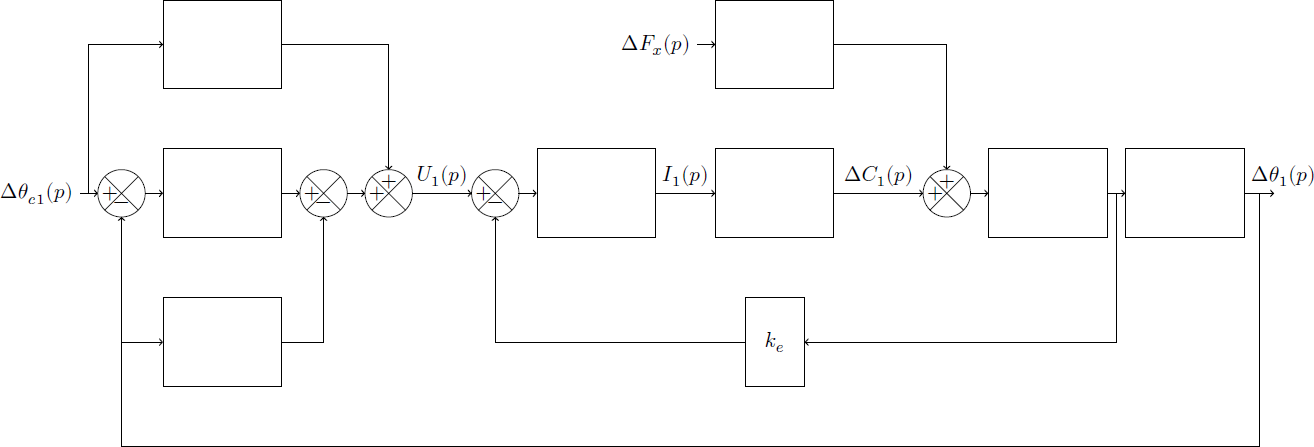
\includegraphics[height=\linewidth]{997_01}}

%\label{fig_2_5}
%\caption{Schéma cinématique du modèle mécanique adopté}
\end{figure}

